\documentclass[xcolor={dvipsnames}]{beamer}
\mode<presentation>
{
  \usetheme{Antibes}      % or try Darmstadt, Madrid, Warsaw, ...
  \usecolortheme{dolphin} % or try albatross, beaver, crane, ...
  \usefonttheme{professionalfonts}  % or try serif, structurebold, ...
  \setbeamertemplate{navigation symbols}{}
  \setbeamertemplate{caption}[numbered]
} 
\usepackage[utf8]{inputenc}
\usepackage[english]{babel}
\usepackage{multirow}
\usepackage{subfigure}
\usepackage{color}
\graphicspath{{/D:/fh/JI/latex/VE230 slides}}
\usepackage{amsmath}
\title[VE230 RC slides week 5]{VE230 RC slides Week 6}
\author{han.fang }
\date{\today}


\begin{document}
\begin{frame}
\titlepage
\end{frame}
\begin{frame}{Materials to cover}
\begin{block}{Today's content}
	\begin{itemize}
		\item Fundamental Postulates
		\item Vector Magnetic Potential
		\item Magnetization and Equivalent Current Densitites
		\item Magnetic Field Intensity, Relative Permeability and
Magnetic circuit
		\item Boundary Conditions for Magnetostatic Fields
	\end{itemize}
\end{block}
\end{frame}
\begin{frame}{Fundamental Postulates}
\begin{table}[H]
  \centering
  \begin{tabular}{c|c|p{5cm}}
  differential form                    & integral form          & Comment            \\
  \hline
  $\nabla\cdot\vec{B}=0$              & $\oint_S\vec{B}\cdot d\vec{s}=0$  & $\vec{B}$ is solenoidal, \newline
  Conservation of magnetic flux: no isolated magnetic charges, no magnetic flow source,\newline flux lines always close upon themselves\\
  \hline
  $\nabla\times\vec{B}=\mu_0\vec{J}$ &  $\oint_C\vec{B}\cdot dl = \mu_0 I$           & Ampere's circuital law
  \end{tabular}
  \end{table}
where $\mu_0$ is the permeability of free space, $\mu_0 = 4\pi\times10^{-7} \quad H/m$.
\end{frame}
\begin{frame}{Fundamental Postulates}
Because the divergence of the curl of any vector field is zero, 
$$
\nabla\cdot \vec{J} = \frac{\nabla\cdot(\nabla\times\vec{B})}{\mu_0} = 0
$$ 

which is consistent with the formula 

$$
\nabla\cdot \vec{J} = \frac{\partial \rho}{\partial t} = 0
$$

for steady current.
\end{frame}
\begin{frame}{Example}
An infinitely long, straight conductor with a circular cross section of radius $b$ carries a steady current $I$. Determine the magnetic flux density both inside and outside the conductor.
\break
\pause
\begin{block}{Answer}
Ampere's circuital law:$\oint_C\vec{B}\cdot dl = \mu_0 I$.  
\end{block}        
\end{frame}
\begin{frame}{Vector Magnetic Potential}
As $\nabla\cdot\vec{B} = 0$, $\vec{B}$ is solenoidal, thus could be expressed as:
\begin{equation}\label{Eq: solenoidal-B-A-relation}
  \vec{B} = \nabla\times \vec{A} \quad (T)
\end{equation}


, where $\vec{A}$ is called the vector magnetic potential.

Magnetic flux $\Phi$:
$$
\Phi = \int_S \vec{B}\cdot d\vec{s} = \oint_C\vec{A}\cdot dl
$$
For Eq~\ref{Eq: solenoidal-B-A-relation}, by doing Laplacian transformation and assume $\nabla\cdot\vec{A} = 0$, vector Poisson's equation:

$$
\nabla^2\vec{A} = -\mu_0\vec{J}
$$

The solution is then 
\begin{equation}\label{Eq: raw-A-J-relation}
  \vec{A} = \frac{\mu_0}{4\pi}\int_{V^\prime} \frac{\vec{J}}{\vec{R}}dv^\prime
\end{equation}
\end{frame}
\begin{frame}{Vector Magnetic Potential}
For a thin wire with cross-sectional area $S$, $dv^\prime = Sdl^\prime$, current flow is entirely along the wire, we then have
$$
\vec{J} dv^\prime = JSdl^\prime = Idl^\prime
$$

Thus, Eq~\ref{Eq: raw-A-J-relation} becomes:
$$
\vec{A} = \frac{\mu_0I}{4\pi} \oint_{C^\prime}\frac{dl^\prime}{R}
$$

Based on this form and properties of differentiation, we can get Biot-Savart law:
$$
\vec{B} = \frac{\mu_0 I}{4\pi}\oint_{C^\prime}\frac{d\vec{l^\prime}\times\vec{a_R}}{R^2}
$$
\end{frame}
\begin{frame}{Vector Magnetic Potential}
The formula for Biot-Savart law could also be written as:
$$
\vec{B} = \oint_{C^\prime}d\vec{B}
$$
and 
$$
d\vec{B} = \frac{\mu_0 I}{4\pi} \left(\frac{d\vec{l^\prime}\times \vec{a_R}}{R^2}\right) = \frac{\mu_0 I}{4\pi} \left(\frac{d\vec{l^\prime}\times \vec{R}}{R^3}\right)
$$

Comment: Biot-Savart law is more difficult to apply than Ampere's circuital law, but Ampere's circuital law cannot be used to determine $\vec{B}$ from $I$ in a circuit if a closed path cannot be found where $\vec{B}$ has a constant magnitude.
\end{frame}
\begin{frame}{Scalar magnetic potential}
If a region is current free, i.e. $\vec{J} = 0$, $$\nabla\times\vec{B} = 0$$,

thus $\vec{B}$ can be expressed as the gradient of a scalar field.

Assume 
\begin{equation}\label{Eq: calculate-B-by-Vm}
  \vec{B} = -\mu_0 \nabla V_m
\end{equation}
, where $V_m$ is called the scalar magnetic potential, the negative sign is conventional, $\mu_0$ is the permeability of free space.

Thus, between two points $P_1, P_2$, 
$$
V_{m2} - V_{m1} = -\int_{P_1}^{P_2} \frac{1}{\mu_0}\vec{B}\cdot dl
$$
\end{frame}
\begin{frame}{Scalar magnetic potential}
If there were magnetic charges with a volume density $\rho_m$ in a volume $V^\prime$, we could find $V_m$ from:
$$
V_m = \frac{1}{4\pi} \int_{V^\prime} \frac{\rho_m}{R}dv^\prime
$$

Then we could obtain $\vec{B}$ by Eq~\ref{Eq: calculate-B-by-Vm}. Note that this is only a mathematical model, isolated magnetic charges have never been found.

For a bar magnet the fictitous magnetic charges $+q_m, -q_m$ assumed to be separated by $d$ (magnetic dipole), the scalar magnetic potential $V_m$ is given by:

$$
V_m = \frac{\vec{m}\cdot\vec{a_R}}{4\pi R^2}
$$
\end{frame}
\begin{frame}{Magnetization and Equivalent Current Densitites}
Define magnetization vector, $\vec{M}$, as
$$
\vec{M} = \lim_{\Delta v\to 0} \frac{\sum_{k=1}^{n\Delta v}\vec{m_k}}{\Delta v}
$$,
which is the volume density of magnetic dipole moment, 

\begin{itemize}
  \item The effect of magnetization is vector is equivalent to both 
  \begin{itemize}
    \item a volume current density:
    $$
    \vec{J_m} = \nabla\times\vec{M}
    $$
    \item a surface current density:
    $$
    \vec{J_{ms}} = \vec{M}\times\vec{a_n}
    $$
  \end{itemize}
  \item Then we can determine $A$ by:
  $$
  \vec{A} = \frac{\mu_0}{4\pi}\int_{V^\prime}\frac{\nabla^\prime\times\vec{M}}{R}dv^\prime + \frac{\mu_0}{4\pi}\oint_{S^\prime}\frac{\vec{M}\times\vec{a_n^\prime}}{R}ds^\prime
  $$
  \item Then we could obtain $\vec{B}$ from $\vec{A}$. 
\end{itemize}
\end{frame}
\begin{frame}{Equivalent Magnetization Charge Densities}
In current-free region, a manetized body may be replaced by 
\begin{enumerate}
  \item an equivalent/fictitous magnetization surface charge density 
  $$
  \rho_{ms} = \vec{M}\cdot\vec{a_n}
  $$ 
  \item an equivalent/fictitous magnetization volume charge density 
  $$
  \rho_m = -\nabla\cdot\vec{M}
  $$ 
\end{enumerate}
\end{frame}
\begin{frame}{Magnetic Field Intensity, Relative Permeability and Magnetic circuit}
Considering the effect of both the internal dipole moment and the induced magnetic moment in a magnetic material, the magnetic field intensity $\vec{H}$ is defined as:
$$
\vec{H} = \frac{\vec{B}}{\mu_0} - \vec{M}
$$

$$
\nabla\times\vec{H} = \vec{J}
$$

directly relates the magnetic field intensity with the density of free charge. 

The integral form of which is then, 
$$
\oint_C\vec{H}\cdot dl = I
$$
\end{frame}
\begin{frame}{Magnetic Field Intensity, Relative Permeability and Magnetic circuit}
It is another form of Ampere's circuital law: the circulation of the magnetic field intensity around any closed path is equal to the free current flowing through the surface bounded by the path.

If the closed path $C$ is chosen to enclose $N$ turns of a winding carrying a current $I$ that excites a magnetic circuit, we have

$$
\oint_C\vec{H}\cdot dl = NI = V_m
$$,

$V_m$ is analogous to electromotive force (emf) and is called magnetomotive force (mmf). 
\end{frame}
\begin{frame}{Magnetic Field Intensity, Relative Permeability and Magnetic circuit}
If we define: 
$$
\vec{M} = \chi_m H
$$,

where $\chi_m$ is magnetic susceptibility, Then
$$
\vec{B} = \mu_0(1+\chi_m)\vec{H} =\mu_0\mu_r\vec{H} =\mu\vec{H}
$$

$$
\vec{H} =\frac{1}{\mu}\vec{B}
$$

$$
\mu_r = 1+\chi_m = \frac{\mu}{\mu_0}
$$

where $\mu_r$ is the relative permeability of the medium. $\mu=\mu_r\mu_0$ is the absolute permeability/permeability. 
\end{frame}
\begin{frame}{Magnetic Field Intensity, Relative Permeability and Magnetic circuit}
If $\vec{B}$ is approximately constant over the core cross section,
$$
R_f = \frac{l_f}{\mu S}
$$,

where $l_f = 2\pi r_o - l_g$ is the length of the ferromagnetic core.

$$
R_g = \frac{l_g}{\mu_0S}
$$

Both the reluctance $R_f$ of the ferromagnetic core and $R_g$ of the air gap have the same formula.


\end{frame}
\begin{frame}{Magnetic Field Intensity, Relative Permeability and Magnetic circuit}
We have the analogous quantities:

\begin{figure}[H]
  \centering
  \includegraphics[width=0.7\linewidth]{analogous-quantities.png}
\end{figure}
And the analysis of the magnetic circuit is similar to the electric circuits.


\end{frame}
\begin{frame}{Magnetic Field Intensity, Relative Permeability and Magnetic circuit}
Similar to Kirchhoff's law, 
$$
\sum_j N_j I_j = \sum_k R_k \Phi_k
$$,

around a closed path in a magnetic circuit, the algebraic sum of ampere-turns is equal to the algebraic sum of the products of the reluctances and fluxes.

$$
\sum_j \Phi_j = 0
$$,

the algebraic sum of all the magnetic fluxes flowing out of a junction in a magnetic circuit is zero.
\end{frame}
\begin{frame}
\begin{block}{Behavior of Magnetic Materials}


\begin{enumerate}
  \item Diamagnetic, if $\mu_r \lesssim 1$ ($\chi_m$ is a very small negative number)
  \item Paramagnetic, if $\mu_r \gtrsim 1$ ($\chi_m$ is a very small positive number)
  \item Ferromagnetic, if $\mu_r >> 1$ ($\chi_m$ is a large positive number)  
\end{enumerate}
\end{block}
\end{frame}
\begin{frame}{Boundary Conditions for Magnetostatic Fields}
\begin{enumerate}
  \item The normal component of $\vec{B}$ is continuous across an interface,
  $$
  B_{1n} = B_{2}
  $$, which is 
  $$
  \mu_1 H_{1n} = \mu_2 H_{2n}
  $$,
  \item The tangential component of the $\vec{H}$ field is discontinuous across an interface where a free surface current exists.
  $$
a_{n2}\times (\vec{H_1} - \vec{H_2}) = \vec{J_s}
  $$
  When the conductivities of both media are finite, currents are defined by volume current densities and free surface currents do not exist on the interface. Hence $\vec{J_s} = 0$, the tangential component of $\vec{H}$ is continuous across the boundary of almost all physical media; it is discontinuous only when an interface with an ideal perfect conductor or a superconductor assumed. 
\end{enumerate}
\end{frame}
\begin{frame}{Boundary Conditions for Magnetostatic Fields}

The magnetic flux lines both inside and outside a cylindrical bar magnet having a uniform axial magnetization $\vec{M} = \vec{a_z}M_0$:

\begin{figure}[H]
  \centering
  \includegraphics[width=0.5\linewidth]{Fig6-21.png}
\end{figure}



\end{frame}
\begin{frame}{Boundary Conditions for Magnetostatic Fields}
Notice here, $\vec{H} = \vec{B}/\mu_0 - \vec{M}$ , $\vec{H} = \vec{B}/\mu_0$ outside the magnet as $\vec{M} = 0$ outside , and $\vec{M}$ is a constant vector inside the magnet.

For current-free regions, $\vec{B} = -\mu\nabla V_m$, thus, 
$$
\nabla^2 V_m = 0
$$
, similar to the Lapace's equation. Similar to what we have discussed in Chapter $4$, we could expect the similar approach here to solve boundary-value problems.
\end{frame}
\begin{frame}
\begin{figure}[H]
	\centering
	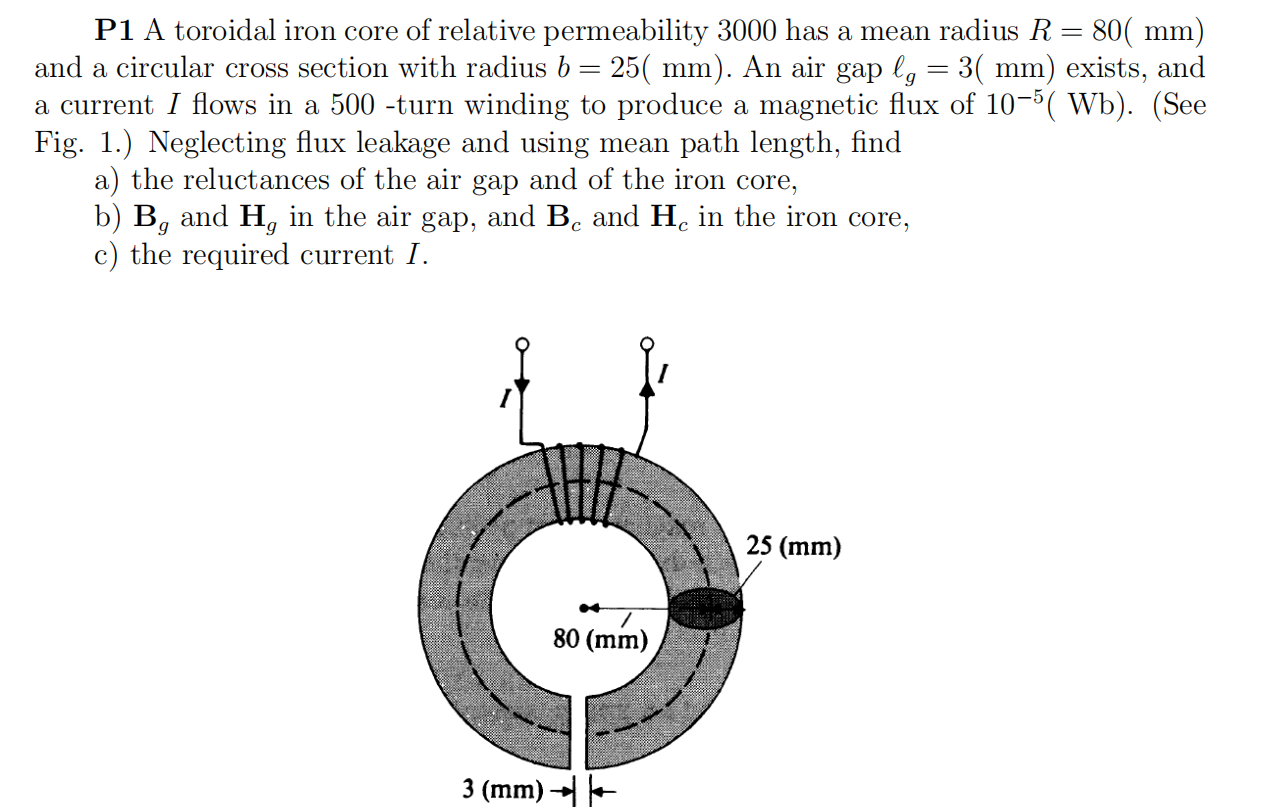
\includegraphics[width=0.9\linewidth]{7_1.png}
\end{figure}
\end{frame}
\begin{frame}
\begin{figure}[H]
	\centering
	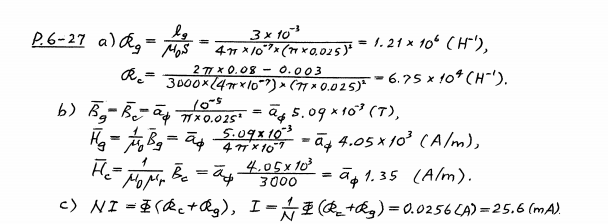
\includegraphics[width=0.9\linewidth]{7_2.png}
\end{figure}
\end{frame}
\begin{frame}
\begin{figure}[H]
	\centering
	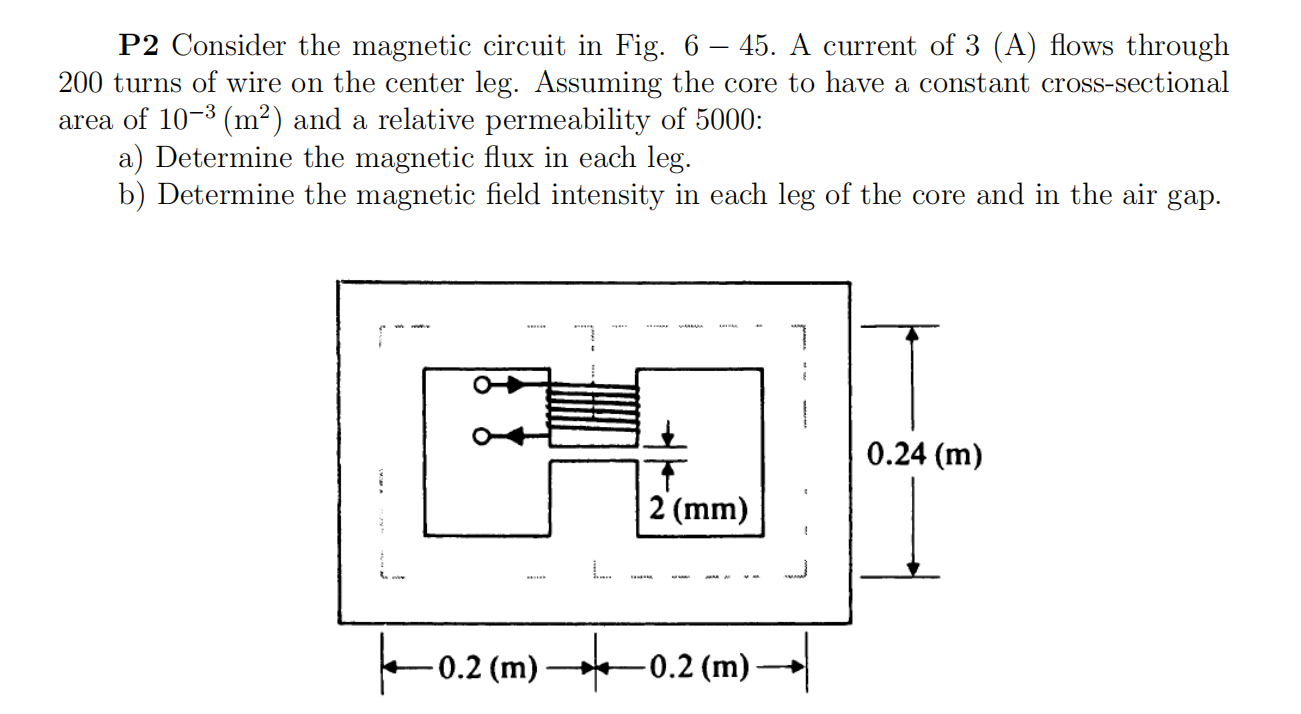
\includegraphics[width=0.9\linewidth]{7_3.png}
\end{figure}
\end{frame}
\begin{frame}
\begin{figure}[H]
	\centering
	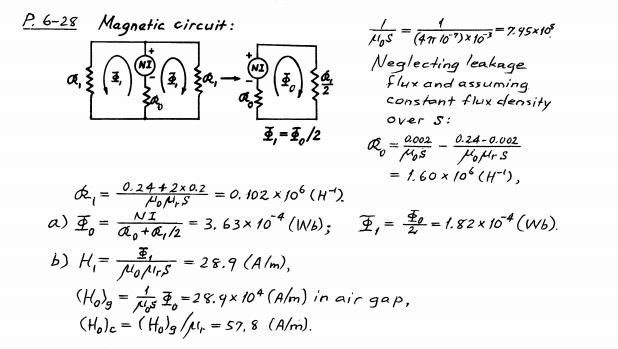
\includegraphics[width=0.9\linewidth]{7_4.png}
\end{figure}
\end{frame}
\begin{frame}
\begin{figure}[H]
	\centering
	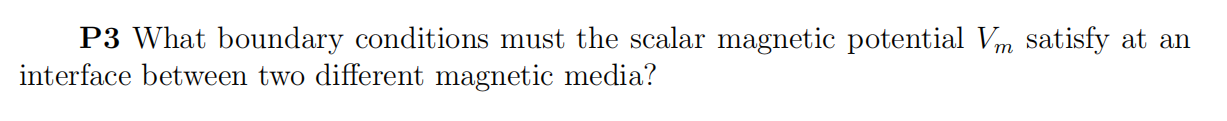
\includegraphics[width=0.9\linewidth]{7_5.png}
\end{figure}
\pause
\begin{figure}[H]
	\centering
	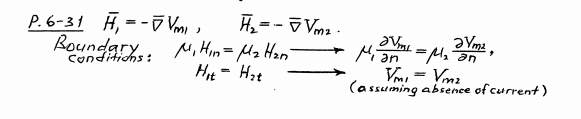
\includegraphics[width=0.9\linewidth]{7_6.png}
\end{figure}
\end{frame}
\begin{frame}
\begin{figure}[H]
	\centering
	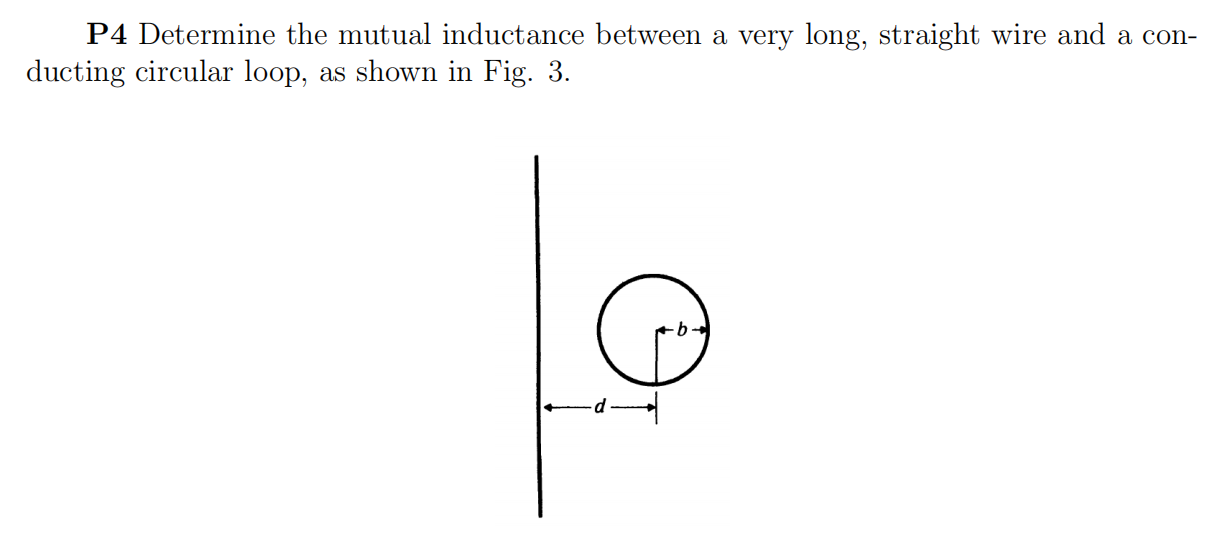
\includegraphics[width=0.9\linewidth]{7_7.png}
\end{figure}
\pause
\begin{figure}[H]
	\centering
	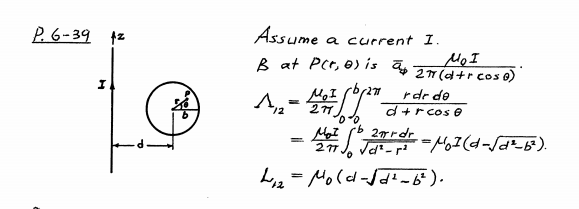
\includegraphics[width=0.9\linewidth]{7_8.png}
\end{figure}
\end{frame}
\begin{frame}
\begin{figure}[H]
	\centering
	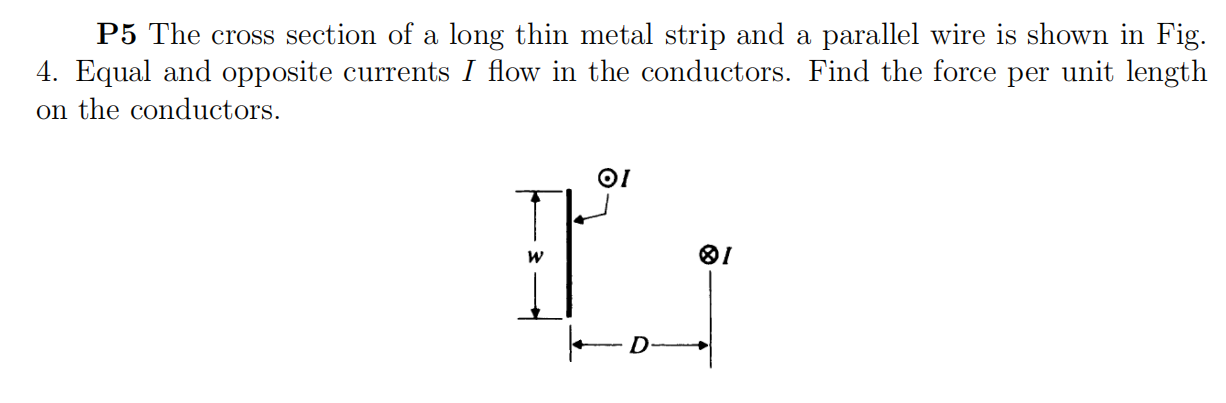
\includegraphics[width=0.9\linewidth]{7_9.png}
\end{figure}
\pause
\begin{figure}[H]
	\centering
	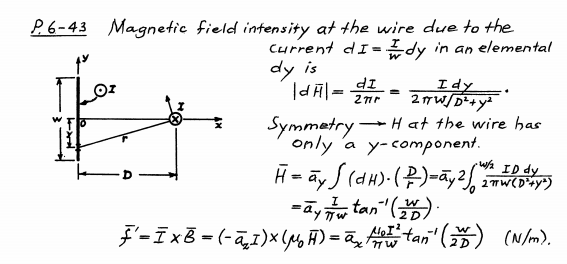
\includegraphics[width=0.9\linewidth]{7_10.png}
\end{figure}
\end{frame}
\begin{frame}
\begin{figure}[H]
	\centering
	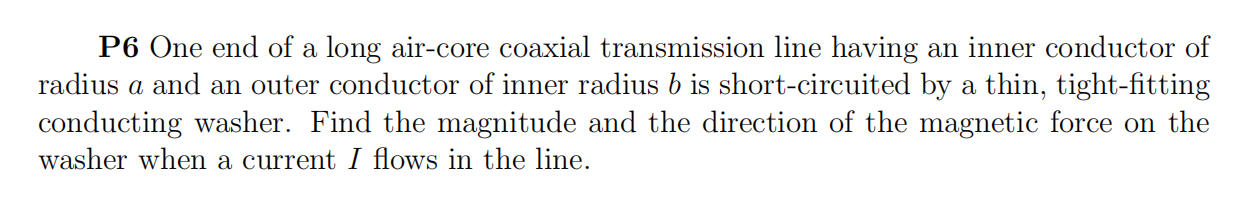
\includegraphics[width=0.9\linewidth]{7_11.png}
\end{figure}
\pause
\begin{figure}[H]
	\centering
	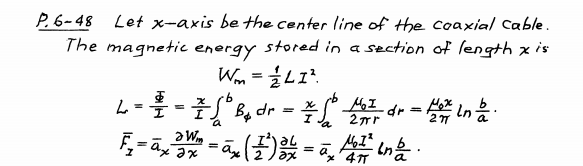
\includegraphics[width=0.9\linewidth]{7_12.png}
\end{figure}
\end{frame}
\begin{frame}
\begin{figure}[H]
	\centering
	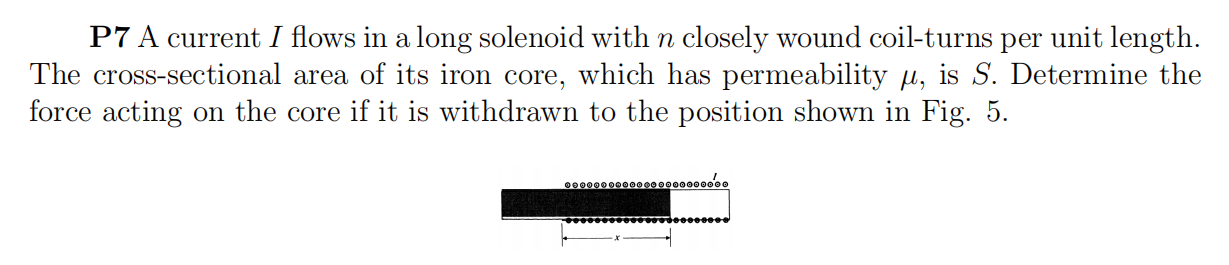
\includegraphics[width=0.9\linewidth]{7_13.png}
\end{figure}
\pause
\begin{figure}[H]
	\centering
	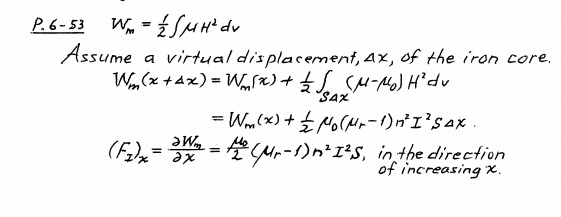
\includegraphics[width=0.9\linewidth]{7_14.png}
\end{figure}
\end{frame}
\end{document}